\chapter{Literature Review }

Deep learning has revolutionized artificial intelligence, enabling significant breakthroughs in various domains. 

The foundation of modern deep learning is well captured by \citeauthor{goodfellow2016deep} in their book \cite{goodfellow2016deep}, where they provide an extensive discussion on neural networks, optimization strategies, and deep architectures. This work serves as a comprehensive resource on the mathematical and practical aspects of deep learning.


In \citeyear{he2016deep}, \citeauthor{he2016deep} introduced the concept of deep residual learning in \cite{he2016deep}. Their work addresses the challenges of training very deep neural networks by introducing residual connections, which help mitigate the vanishing gradient problem. By using identity mappings, the proposed residual networks (ResNets) allow for more effective gradient flow, leading to significant improvements in deep model training. Their architecture achieved state-of-the-art performance on benchmark datasets such as ImageNet, demonstrating the importance of deeper networks in advancing computer vision tasks.

\section{Mathematical Formulation}
The research problem can be expressed as:
\begin{equation}
	E = mc^2
\end{equation}
where $E$ is energy, $m$ is mass, and $c$ is the speed of light.


\section{Tables and Figures}
Table~\ref{tab:example} presents some sample data.

\begin{table}[h]
	\centering
	\begin{tabular}{l c c}
		\toprule
		Category & Value 1 & Value 2 \\
		\midrule
		A & 10 & 20 \\
		B & 15 & 25 \\
		C & 20 & 30 \\
		\bottomrule
	\end{tabular}
	\caption{An example table.}
	\label{tab:example}
\end{table}

Figure~\ref{fig:example} illustrates an example image.


\begin{table}[h]
	\centering
	\rowcolors[\hline]{2}{green!30}{yellow!50} %alternate row colors starting at row 2
	 \arrayrulecolor{red} % border color
	 \setlength\arrayrulewidth{1.2pt} %  border size
	\begin{tabular}{|l| c| c|}
		\hline
	\rowcolor{pink} 	Category & Value 1 & Value 2 \\
		\hline
		  A & 10 & 20 \\ \hline 
		 B & 15 & 25 \\ \hline 
		   C & 20 & 30 \\ 
		\hline
				   D & 10 & 50 \\ 
		\hline
				   E & 50 & 80 \\ 
		\hline
	\end{tabular}
	\caption{An example table with some colors.}
	\label{tab:example2}
\end{table}


\begin{figure}[h]
	\centering
	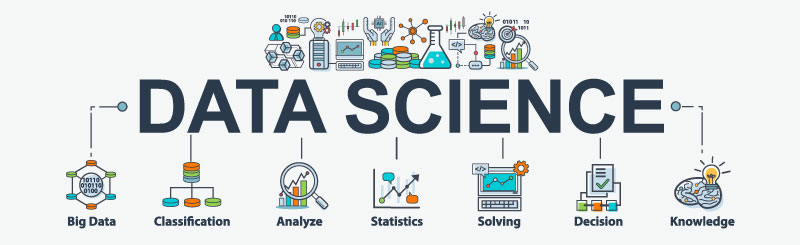
\includegraphics[width=0.75\textwidth]{img/data-science}
	\caption{An example figure.}
	\label{fig:example}
\end{figure}

\section{Enumerations}
Important points to consider:
\begin{enumerate}
	\item First point.
	\item Second point.
	\item Third point.
\end{enumerate}

Enumerations with alpha numerics.
\begin{enumerate}[label={(\alph*)}]
	\item First point.
	\item Second point.
	\item Third point.
\end{enumerate}


Roman Enumerates.

\begin{enumerate}[label={(\roman*)}]
	\item First point.
	\item Second point.
	\item Third point.
\end{enumerate}